%%%%%%%%%%%%%%%%%%%%%%%%%%%%%%%%%%%%%%%%%%%%%%%%
% Template TCMN data sheet version 3
% 
% Alberto Sanchez asanchezrodelgo@ifc.org Dec 2015
%%%%%%%%%%%%%%%%%%%%%%%%%%%%%%%%%%%%%%%%%%%%%%%%
\documentclass{article}\usepackage[]{graphicx}\usepackage[]{color}
%% maxwidth is the original width if it is less than linewidth
%% otherwise use linewidth (to make sure the graphics do not exceed the margin)
\makeatletter
\def\maxwidth{ %
  \ifdim\Gin@nat@width>\linewidth
    \linewidth
  \else
    \Gin@nat@width
  \fi
}
\makeatother

\definecolor{fgcolor}{rgb}{0.345, 0.345, 0.345}
\newcommand{\hlnum}[1]{\textcolor[rgb]{0.686,0.059,0.569}{#1}}%
\newcommand{\hlstr}[1]{\textcolor[rgb]{0.192,0.494,0.8}{#1}}%
\newcommand{\hlcom}[1]{\textcolor[rgb]{0.678,0.584,0.686}{\textit{#1}}}%
\newcommand{\hlopt}[1]{\textcolor[rgb]{0,0,0}{#1}}%
\newcommand{\hlstd}[1]{\textcolor[rgb]{0.345,0.345,0.345}{#1}}%
\newcommand{\hlkwa}[1]{\textcolor[rgb]{0.161,0.373,0.58}{\textbf{#1}}}%
\newcommand{\hlkwb}[1]{\textcolor[rgb]{0.69,0.353,0.396}{#1}}%
\newcommand{\hlkwc}[1]{\textcolor[rgb]{0.333,0.667,0.333}{#1}}%
\newcommand{\hlkwd}[1]{\textcolor[rgb]{0.737,0.353,0.396}{\textbf{#1}}}%

\usepackage{framed}
\makeatletter
\newenvironment{kframe}{%
 \def\at@end@of@kframe{}%
 \ifinner\ifhmode%
  \def\at@end@of@kframe{\end{minipage}}%
  \begin{minipage}{\columnwidth}%
 \fi\fi%
 \def\FrameCommand##1{\hskip\@totalleftmargin \hskip-\fboxsep
 \colorbox{shadecolor}{##1}\hskip-\fboxsep
     % There is no \\@totalrightmargin, so:
     \hskip-\linewidth \hskip-\@totalleftmargin \hskip\columnwidth}%
 \MakeFramed {\advance\hsize-\width
   \@totalleftmargin\z@ \linewidth\hsize
   \@setminipage}}%
 {\par\unskip\endMakeFramed%
 \at@end@of@kframe}
\makeatother

\definecolor{shadecolor}{rgb}{.97, .97, .97}
\definecolor{messagecolor}{rgb}{0, 0, 0}
\definecolor{warningcolor}{rgb}{1, 0, 1}
\definecolor{errorcolor}{rgb}{1, 0, 0}
\newenvironment{knitrout}{}{} % an empty environment to be redefined in TeX

\usepackage{alltt}
%%%%%%%%%%%%%% package declaration %%%%%%%%%%%%%%%%%%%%%
\usepackage[top=0.3in, bottom=0.1in, left=0.5in, right=0.6in]{geometry}
\usepackage{graphicx} % to load images
\usepackage[export]{adjustbox} % add alignment to includegraphics
\usepackage[font=small]{caption}
\usepackage{xcolor} % color text
\usepackage{tabularx} % to adjust table width, etc. 
\usepackage{titlesec} % format titles and headers
\usepackage{sectsty} % format sections & subsections
\usepackage{booktabs} % For \toprule, \midrule and \bottomrule
\usepackage[colorlinks = true,
            linkcolor = blue,
            urlcolor  = blue,
            citecolor = blue,
            anchorcolor = blue]{hyperref} % to include hyperlinks in the doc
\sectionfont{\fontsize{16}{15}\selectfont\raggedright} % formats title newsletter (section) 
\subsectionfont{\fontsize{14}{12}\selectfont\raggedright} % formats title newsletter (section)
%%%%%%%%%%%%%%%%%%%%%%%%%%%%%%%%%%%%%%%%%%%%%%%%%%%%%%%%%%%%%%%%%%%%%%%%%%%%%%%%%%%
%
%%%%%%%%%%%%%%%%%%%%%%%%%%%%%%%%%%%%% BEGIN DOCUMENT %%%%%%%%%%%%%%%%%%%%%%%%%%%%%%
\IfFileExists{upquote.sty}{\usepackage{upquote}}{}
\begin{document}

%

%%%%%%%%%%%%%%%% PAGE 1 %%%%%%%%%%%%%%%%%%%
%World Bank logo and TCMN branding
\begin{figure}
  \vspace{-3ex} % move up this figure
  \hspace{-7ex} % move left this figure
  \includegraphics[width=5cm]{/Users/asanchez3/shinyTCMN/www/wb_logo_background.png}
\end{figure}
\begin{figure}
  \begin{minipage}[t]{0.99\textwidth} % top section
      \vspace{-30ex}
      \hspace{-2ex}
      \raggedright{\includegraphics[width=5.5cm,right]{/Users/asanchez3/shinyTCMN/www/TC_snapshots_data.png}}
  %  {\color{white!70!black}\noindent\makebox[\linewidth]{\rule{20cm}{0.3pt}}} % horiz line
  \end{minipage}
\end{figure}
%
%%%% Macro Indicators
\begin{minipage}[t]{0.99\textwidth} % top section
  \vspace{-1.5cm}
  \begin{minipage}[c]{0.36\textwidth} 
    \begin{minipage}[c]{0.28\textwidth} % flag
      \includegraphics[width=1.2cm,height=1.2cm]{/Users/asanchez3/shinyTCMN/www/RU.png}
    \end{minipage}
    \begin{minipage}[c]{0.70\textwidth} % Country name
      \section*{\color{blue!40!black}Russian Federation}
    \end{minipage}
  \end{minipage}
  \begin{minipage}[c]{0.63\textwidth} % key macro table 
    % Table 1
    \centering
    \resizebox{\textwidth}{!}{
% latex table generated in R 3.2.2 by xtable 1.7-4 package
% Tue May 31 10:59:13 2016
{\LARGE
\begin{tabular}{>{\centering}p{1.5in}>{\centering}p{1.5in}>{\centering}p{1.5in}>{\centering}p{1.5in}>{\centering}p{1.5in}>{\centering}p{1.5in}>{\centering}p{1.5in}l}
  GDP (US\$ billions) (2017) & Population (millions) (2017) & Land area (sq. km) (2015) & Income per capita (current US\$) (2017) & Poverty rate (2012) \large{[1]} & Unemployment rate (2016) & Ease of Doing Business Rank (2016) &  \\ 
       1,488.16 &        142.50 & 16,376,870.00 &     10,443.58 &          0.04 &          6.50 &         51.00 &  \\ 
  \end{tabular}
}

    }
  \end{minipage}  
\end{minipage} % end top section

\begin{minipage}[b]{0.99\textwidth} % macro indicators main table
  %\vspace*{0.5cm}
  %\vspace{+3ex}
  \begin{minipage}[t]{0.99\textwidth}

    \begin{minipage}[c]{0.875\textwidth}
      \begin{flushleft}  
      {\color{white!30!blue} \textbf{\small Macro Indicators}}
      \end{flushleft} 
      \vspace*{-0.4cm}
      % Table 2
      \centering
      \resizebox{\textwidth}{!}{
% latex table generated in R 3.2.2 by xtable 1.7-4 package
% Tue May 31 10:59:13 2016
{\Large
\begin{tabular}{>{\raggedright}p{6in}r>{\raggedleft}p{0.8in}>{\raggedleft}p{0.8in}>{\raggedleft}p{0.8in}>{\raggedleft}p{0.8in}>{\raggedleft}p{0.8in}l}
  & Avg 2003-2012 & 2013 & 2014 & 2015 & 2016 & 2017 &  \\ 
  \hline
GDP growth (annual \%) &   4.75 &   1.34 &   0.64 &  -3.80 &  -0.60 &   1.50 &  \\ 
  Current account balance &   8.10 &   1.68 &   3.15 &   7.71 &   6.76 &   4.96 &  \\ 
  Fiscal balance (\% of GDP) &   2.55 &  -1.28 &  -1.18 &  -4.28 &  -2.38 &  -0.88 &  \\ 
  Remittances, received (\% of GDP) \large{[1]} &   0.37 &   0.32 &   0.42 & --- & --- & --- &  \\ 
  General government gross debt \large{[3]} &  15.52 &  13.07 &  16.33 &  17.71 &  18.39 & --- &  \\ 
  Real Effective Exchange Rate (2010=100) &  87.84 & 108.28 &  98.15 &  77.69 &  83.57 &  90.02 &  \\ 
  Consumer Price Index, annual percent change &  11.61 &   6.75 &   7.82 &  15.50 &   7.50 &   5.00 &  \\ 
  \end{tabular}
}

      }
    \end{minipage}
    \begin{minipage}[c]{0.11\textwidth}
      \vspace*{+0.8cm}


{\centering 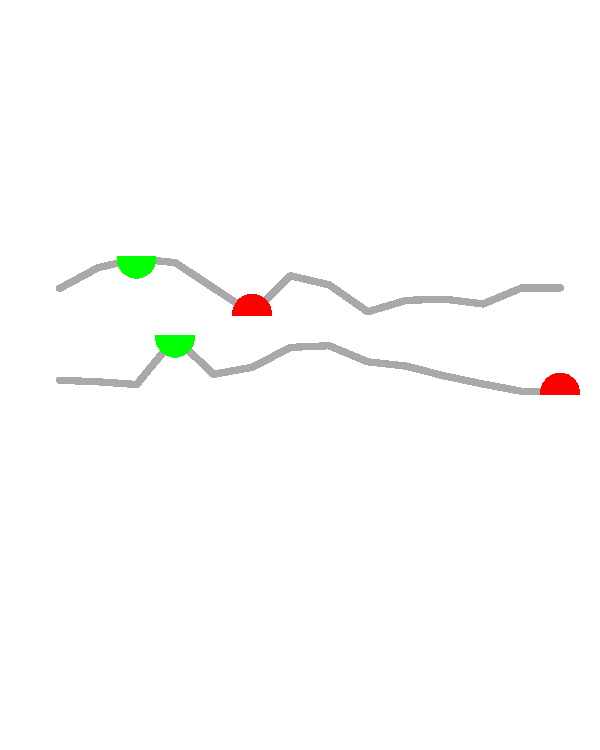
\includegraphics[width=\maxwidth]{figure/createSparklines_macro-1} 

}



      \vspace*{-0.5cm}
    \end{minipage}
    
    %\vspace*{-0.4cm}
    \begin{minipage}[c]{0.875\textwidth}
      \begin{flushleft}  
      {\color{white!30!blue} \textbf{\small Investment indicators}}
      \end{flushleft} 
      \vspace*{-0.4cm}
      % Table 2
      \centering
      \resizebox{\textwidth}{!}{
% latex table generated in R 3.2.2 by xtable 1.7-4 package
% Tue May 31 10:59:13 2016
{\Large
\begin{tabular}{>{\raggedright}p{6in}r>{\raggedleft}p{0.8in}>{\raggedleft}p{0.8in}>{\raggedleft}p{0.8in}>{\raggedleft}p{0.8in}>{\raggedleft}p{0.8in}l}
  & Avg 2003-2012 & 2013 & 2014 & 2015 & 2016 & 2017 &  \\ 
  \hline
Gross domestic investment (\% GDP) & 18.8 & 22.5 & 21.9 & 20.8 & 20.7 & 21.5 &  \\ 
  Gross domestic investment, of w: Private investment (\% GDP) \large{[1]} & 22.4 & 22.8 & 20.3 & --- & --- & --- &  \\ 
  Inward FDI (\% of GDP) \large{[2]} &  2.9 &  3.3 &  1.1 & --- & --- & --- &  \\ 
  Inward FDI, \% of private investment \large{[2]} & 13.9 & 15.4 &   NA & --- & --- & --- &  \\ 
  \end{tabular}
}

      }
    \end{minipage}
    \begin{minipage}[c]{0.11\textwidth}
      \vspace*{+0.8cm}


{\centering 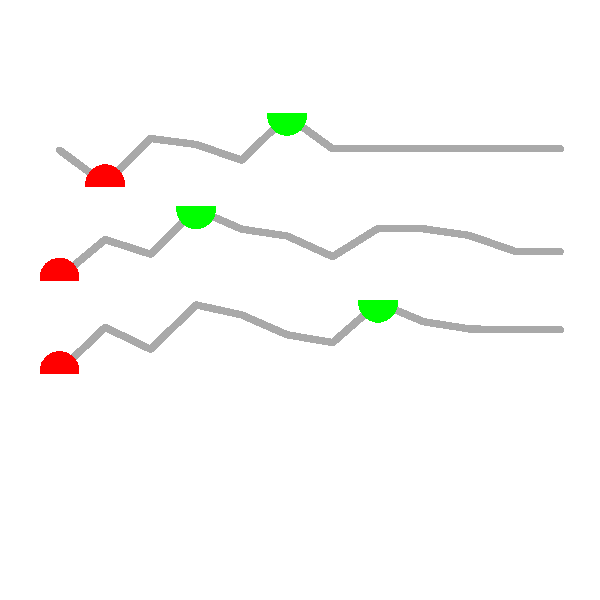
\includegraphics[width=\maxwidth]{figure/createSparklines_invest-1} 

}



      \vspace*{-0.5cm}
    \end{minipage}
    
    %\vspace*{-0.4cm}
    \begin{minipage}[c]{0.875\textwidth}
      \begin{flushleft}  
      {\color{white!30!blue} \textbf{\small Trade Indicators}}
      \end{flushleft} 
      \vspace*{-0.4cm}
      % Table 2
      \centering
      \resizebox{\textwidth}{!}{
% latex table generated in R 3.2.2 by xtable 1.7-4 package
% Tue May 31 10:59:13 2016
{\Large
\begin{tabular}{>{\raggedright}p{6in}r>{\raggedleft}p{0.8in}>{\raggedleft}p{0.8in}>{\raggedleft}p{0.8in}>{\raggedleft}p{0.8in}>{\raggedleft}p{0.8in}l}
  & Avg 2003-2012 & 2013 & 2014 & 2015 & 2016 & 2017 &  \\ 
  \hline
Total Trade in Goods and Services (\% of GDP, real terms) &  48.60 &  57.09 &  54.76 &  52.03 &  53.13 &  54.31 &  \\ 
  Trade balance (\% GDP, real terms) &  15.28 &   7.25 &   9.13 &  15.04 &  15.36 &  14.86 &  \\ 
  Exports, Goods and Services, annual percent change (real terms) &   5.28 &   4.58 &  -0.08 &   1.00 &   1.50 &   2.50 &  \\ 
  Imports, Goods and Services, annual percent change (real terms) &  14.76 &   3.84 &  -7.87 & -22.00 &   1.50 &   6.00 &  \\ 
  Total reserves in months of imports \large{[1]} &  12.25 &  10.34 &   8.53 & --- & --- & --- &  \\ 
  \end{tabular}
}

      }
    \end{minipage}
    \begin{minipage}[c]{0.11\textwidth}
      \vspace*{+0.8cm}


{\centering 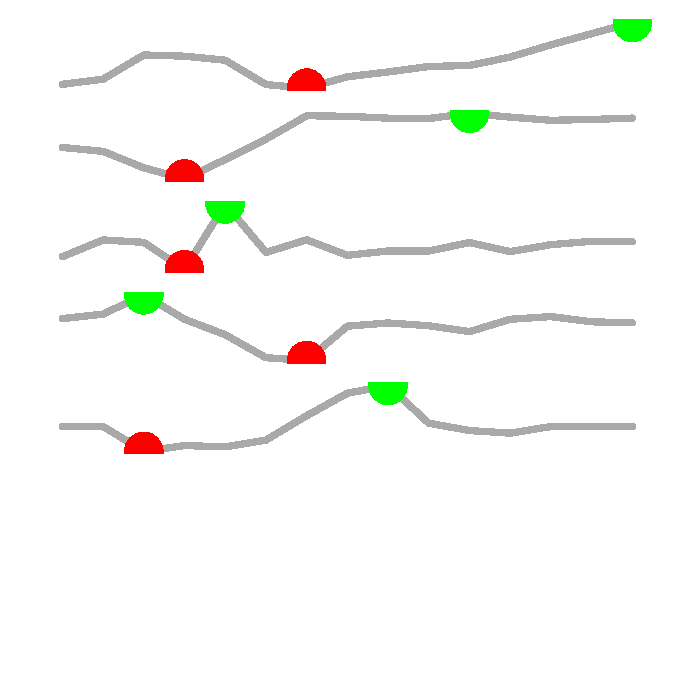
\includegraphics[width=\maxwidth]{figure/createSparklines_trade-1} 

}



      \vspace*{-0.4cm}
    \end{minipage}
  \\[3pt]
\raggedright{\footnotesize{\href{http://www.worldbank.org/en/topic/macroeconomics/overview}{Sources: MFM note}{,} \href{http://data.worldbank.org/data-catalog/world-development indicators}{[1] World Development Indicators (WDI)}{,} \href{http://unctadstat.unctad.org/wds/ReportFolders/reportFolders.aspx}{[2] UNCTADSTAT}{,} \href{https://www.imf.org/external/pubs/ft/weo/2015/02/weodata/index.aspx}{[3] World Economic Outlook (WEO)}}}
  \end{minipage} 
%\end{minipage}    
  \begin{minipage}[b]{\textwidth} % macro charts
  \vspace{+3ex}
    \begin{minipage}[c]{0.49\textwidth} % imports/exports 
    \center{\color{blue!50!black} \textbf{\small Goods Export and Import \\ volume growth, 2012-2015}}


{\centering 
\includegraphics[width=\maxwidth]{figure/ExpImp_HF-1} 

}



    \vspace*{-0.3cm}
    %\hspace*{0.5cm} 
    \raggedright{\footnotesize{\href{http://web.worldbank.org/WBSITE/EXTERNAL/EXTDEC/EXTDECPROSPECTS/0,,menuPK:476941~pagePK:51084723~piPK:51084722~theSitePK:476883,00.html}{Source: Development Prospects Group (DECPG)}}}
    \end{minipage}
    \begin{minipage}[c]{0.49\textwidth} % gdp value added
    \center{\color{blue!50!black} \textbf{\small Gross Value Added by \\ Economic Activity 2013 \footnotesize(\% GDP)}}


{\centering 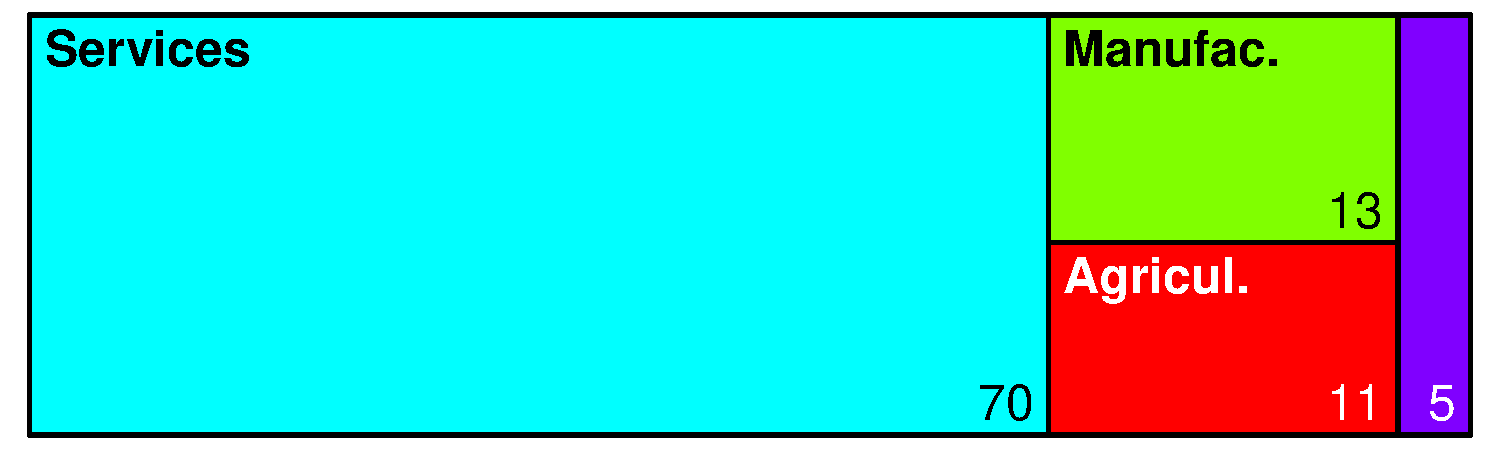
\includegraphics[width=\maxwidth]{figure/GVA_Treemap-1} 

}



   %\vspace*{-0.3cm}
   %\hspace*{0.5cm} 
   \raggedright{\footnotesize{\href{http://data.worldbank.org/data-catalog/world-development indicators}{Source: World Development Indicators (WDI)}}}
    \end{minipage}
  \end{minipage}  
\end{minipage}   
 
%%%% Exports Imports and DB
\begin{minipage}[b]{0.99\textwidth}
  \vspace{0.8cm}
   \begin{minipage}[c]{0.44\textwidth} 
    %\vspace*{-0.2cm}
    \begin{minipage}[t]{0.99\textwidth} 
      {\color{blue!50!black} \textbf{\small Top 5 Exports by \% of Total Value, 2015}}
      %\vspace{3ex}
      \\[6pt]
      \centering
      \resizebox{\textwidth}{!}{%


{\centering 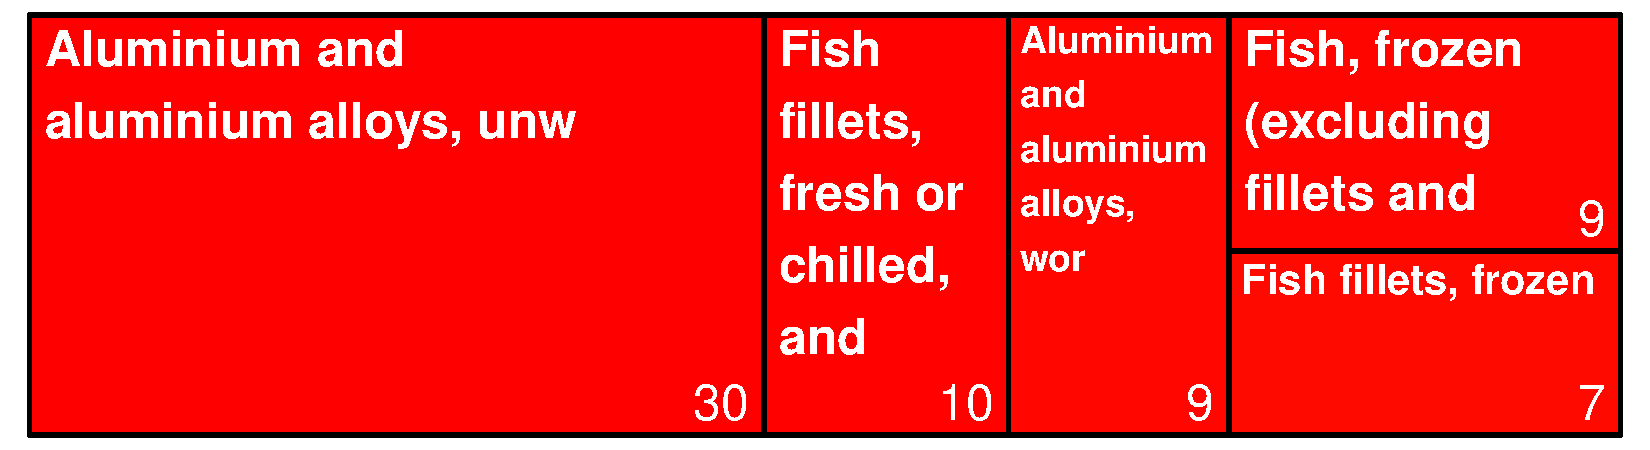
\includegraphics[width=\maxwidth]{figure/ImpExp_Treemap-2-1} 

}



      }
      \end{minipage}
      \\[14pt]
      \begin{minipage}[t]{0.99\textwidth} 
      {\color{blue!50!black} \textbf{\small Imports Categories by \% of Total Value, 2015}}
      \\[6pt]
      \centering
      \resizebox{\textwidth}{!}{%


{\centering 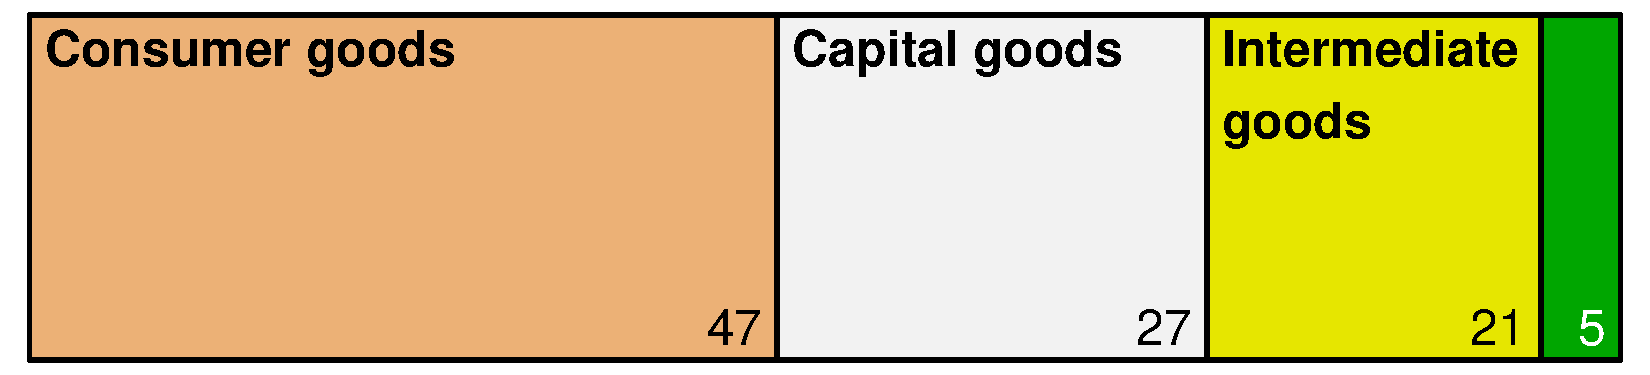
\includegraphics[width=\maxwidth]{figure/ImpExp_Treemap-1-1} 

}



      }
      \end{minipage}
      \\[10pt]
    %\hspace*{0.5cm}
    \footnotesize{\href{http://wits.worldbank.org}{Source: World Integrated Trade Solution (WITS)}} 
    \end{minipage}
    \begin{minipage}[c]{0.56\textwidth} % Doing Business table
    %\vspace*{-0.1cm}
    %\begin{flushleft}
      \center {\color{blue!50!black}\textbf{\small Doing Business 2015 \\ \footnotesize Distance to Frontier (DTF) and Rank}}
    %\end{flushleft}
    \\[18pt]
    \centering
      \resizebox{\textwidth}{!}{%
% latex table generated in R 3.2.2 by xtable 1.7-4 package
% Tue May 31 10:59:14 2016
{\large
\begin{tabular}{lrrr|rrrr}
  &  & DTF &  &  & Rank &  &  \\ 
  &  2015 &  2016 &  Change & 2015 & 2016 & Change &  \\ 
   \hline
\textbf{Ease of Doing Business} & \textbf{69.26} & \textbf{70.99} & \textbf{\color{green}{1.73}} & \textbf{54} & \textbf{51} & \textbf{\color{green}{3}} &  \\ 
  Dealing with Construction Permits & 65.17 & 65.23 & \color{green}{0.06} & 117 & 119 & \color{red}{-2} &  \\ 
  Enforcing Contracts & 78.56 & 78.56 & 0 & 5 & 5 & 0 &  \\ 
  Getting Credit & 55 & 65 & \color{green}{10} & 61 & 42 & \color{green}{19} &  \\ 
  Getting Electricity & 77.89 & 84.22 & \color{green}{6.33} & 53 & 29 & \color{green}{24} &  \\ 
  Paying Taxes & 80.63 & 81.6 & \color{green}{0.97} & 50 & 47 & \color{green}{3} &  \\ 
  Protecting Minority Investors & 56.67 & 56.67 & 0 & 64 & 66 & \color{red}{-2} &  \\ 
  Registering Property & 90.12 & 90.51 & \color{green}{0.39} & 8 & 8 & 0 &  \\ 
  Resolving Insolvency & 59.06 & 58.39 & \color{red}{-0.67} & 44 & 51 & \color{red}{-7} &  \\ 
  Starting a Business & 92.17 & 92.35 & \color{green}{0.18} & 34 & 41 & \color{red}{-7} &  \\ 
  Trading Across Borders & 37.39 & 37.39 & 0 & 169 & 170 & \color{red}{-1} &  \\ 
  \end{tabular}
}

      }
    \\[15pt]
     %\hspace*{0.5cm} 
     \raggedright{\footnotesize{\href{http://www.doingbusiness.org/data}{Source: Doing Busines Report 2015}}}
    \end{minipage}
\end{minipage}

% \vspace{+3ex}
% {\color{blue!50!white}\noindent\makebox[\linewidth]{\rule{18cm}{0.3pt}}} % horiz line
% \begin{minipage}[c]{0.99\textwidth}
%   \hspace*{-0.4cm}\raggedleft{\color{white!40!black} \footnotesize TRADE AND COMPETITIVENESS MONITORING NOTE - UPDATED} 
%   %month year}
% \end{minipage}

\newpage
%%%%%%%%%%%%%%%% PAGE 2 %%%%%%%%%%%%%%%%%%%

\begin{minipage}[t]{0.99\textwidth}
  \vspace{0.5cm}
  \begin{minipage}[c]{0.48\textwidth} % WEF Radar
    \center{\color{blue!50!black} \textbf{WEF Competitiveness Indicators \\ \footnotesize(Scale 1-7, 7=best)}}
    \vspace*{-0.6cm}


{\centering 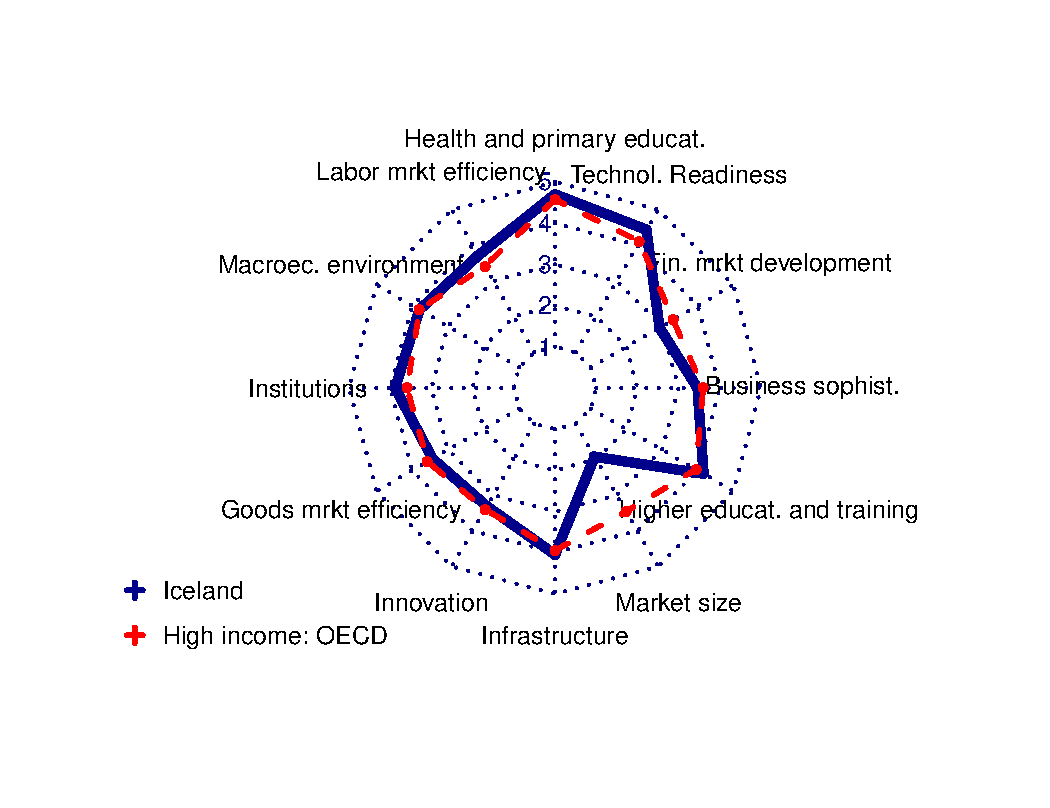
\includegraphics[width=\maxwidth]{figure/WEFradar-1} 

}



    \vspace*{-0.6cm} 
    \hspace*{0.3cm} \raggedright\footnotesize{\href{http://www.weforum.org/global-competitiveness-report-2015-2016}{Source: WEF Global Competitiveness Report 2015}}
  \end{minipage}
  \begin{minipage}[c]{0.50\textwidth} % LPI chart
  %\vspace*{0.5cm}
  \center {\color{blue!50!black} \textbf{Logistics Performance Index \\ \footnotesize(Scale 1-5, 5=best)}}
    \vspace*{0.4cm}


{\centering 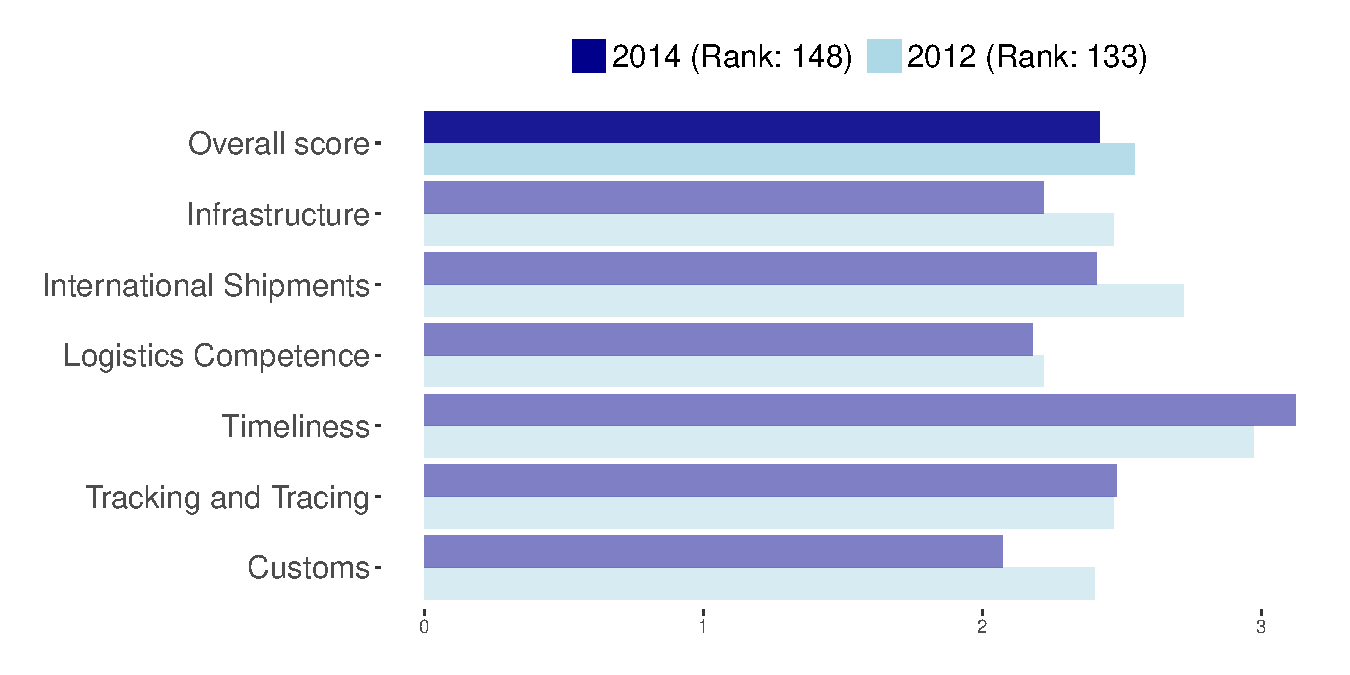
\includegraphics[width=\maxwidth]{figure/LPIindicators-1} 

}



  %\hspace*{0.5cm} 
  \raggedright\footnotesize{\href{http://lpi.worldbank.org}{Source: Logistics Performance Index (World Bank)}}
  \end{minipage}
\end{minipage}  

\begin{minipage}[b]{0.99\textwidth}
  \begin{minipage}[c]{0.50\textwidth} % WGI chart
    \vspace*{0.8cm}
    \center {\color{blue!50!black} \textbf{World Governance indicators \\ \footnotesize(Std. score, High=best)}}
    \vspace*{0.3cm}


{\centering 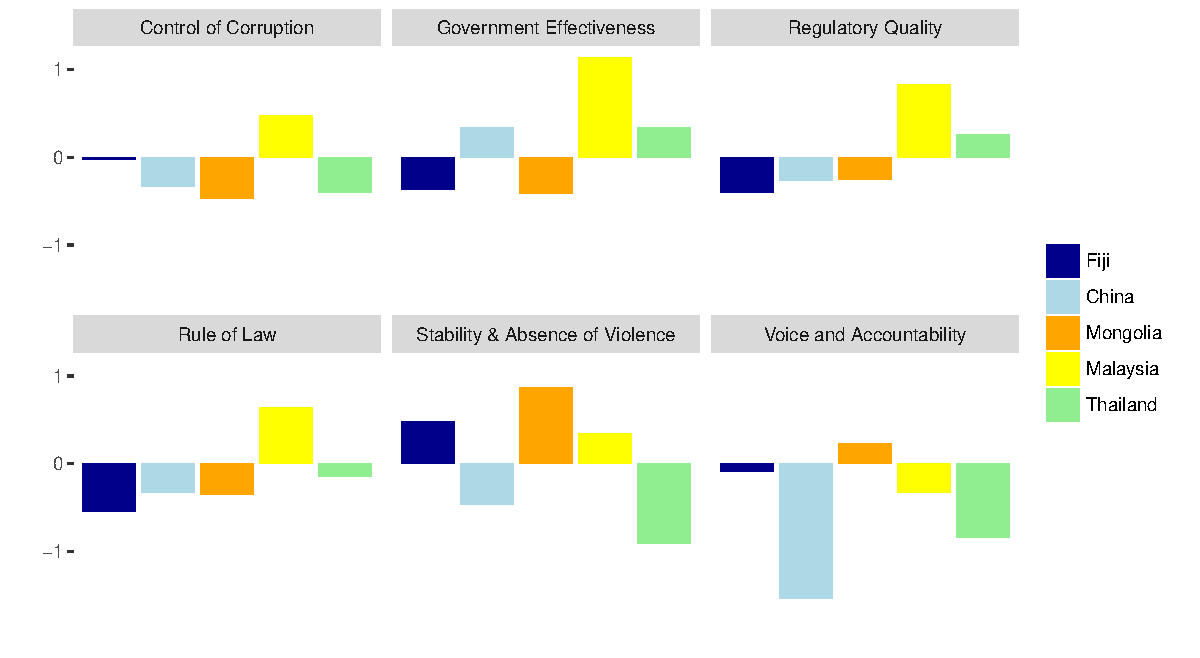
\includegraphics[width=\maxwidth]{figure/WGIindicators-1} 

}



    \vspace*{-0.6cm} 
    \hspace*{0.3cm} \raggedright\footnotesize{\href{http://data.worldbank.org/data-catalog/worldwide-governance-indicators}{Source: Worldwide Governance Indicators}}
  \end{minipage}
  \begin{minipage}[c]{0.48\textwidth} % Trade Policy table
    \vspace*{0.4cm}
  %\begin{flushleft}
    {\color{blue!50!black} \textbf{Trade Policy}}
  %\end{flushleft} 
  %\vspace*{0.2cm}
    \\[20pt]
    \centering
    \resizebox{\textwidth}{!}{%
% latex table generated in R 3.2.2 by xtable 1.7-4 package
% Tue May 31 10:59:15 2016
{\Large
\begin{tabular}{lrrr}
  & 2010 & 2015 &  \\ 
  \hline
Applied Tariff (Incl. Prefers. and Trade-Weighted) & 7.1 & 5 &  \\ 
  Binding (\%) & 100.0 & --- &  \\ 
  Dispersion (Standard Deviation) & 10.0 & 6 &  \\ 
  MFN Tariff (Agriculture) & 11.8 & 8 &  \\ 
  MFN Tariff (Non-Agriculture) & 8.5 & 6.9 &  \\ 
  MFN Tariff (Simple Average) & 9.0 & 7 &  \\ 
  \end{tabular}
}

    }
    \\[20pt]
    %\hspace*{0.5cm} 
    \raggedright{\footnotesize{\href{http://wits.worldbank.org}{Sources: WITS}{, }\href{http://stat.wto.org/CountryProfile/WSDBCountryPFHome.aspx?Language=E}{[1] WTO Trade Profiles}}}
  \end{minipage}
\end{minipage}

\vspace{+8ex}
%\hspace*{0.2cm}\subsection*{\color{white!50!black}Private Sector's Views}
\hspace*{0.1cm} \raggedright{\color{white!50!black}\Large Private Sector View}

\vspace*{-0.2cm}
{\color{white!30!black}\noindent\makebox[\linewidth]{\rule{18cm}{0.2pt}}} % horiz line

\begin{minipage}[b]{0.99\textwidth}
\vspace*{+0.6cm}
  \begin{minipage}[c]{0.02\textwidth}
  \hspace*{+0.1cm}
  \end{minipage}
  \begin{minipage}[c]{0.97\textwidth} 
    \begin{flushleft}  
      {\color{blue!50!black} \textbf{Enterprise Survey 2012}}
    \end{flushleft}  
    \vspace*{-0.4cm}
    \centering
    \resizebox{\textwidth}{!}{%
% latex table generated in R 3.2.2 by xtable 1.7-4 package
% Tue May 31 10:59:15 2016
{\Large
\begin{tabular}{lrrl}
  & All Countries & Russian Federation &  \\ 
  \hline
Number of electrical outages in a typical month & 6.30 & 0.30 &  \\ 
  Percent of firms with a bank loan/line of credit & 35.20 & 21.60 &  \\ 
  Proportion of investments financed by banks (\%) & 14.60 & 6.30 &  \\ 
  Proportion of investments financed internally (\%) & 71.20 & 84.30 &  \\ 
  Senior management time spent dealing with the requirements of government regulation (\%) & 10.00 & 14.70 &  \\ 
  \end{tabular}
}

    }
    \\[8pt]
    %\hspace*{0.3cm} 
    \raggedright{\footnotesize{\href{https://www.enterprisesurveys.org/data}{Source: Enterprise Survey 2012}}}
  \end{minipage} 

  \begin{minipage}[b]{0.99\textwidth} 
    \vspace{+4ex}
    \begin{minipage}[c]{0.49\textwidth} % top 5 constraints ES
      \center{\color{blue!50!black} \textbf{Top 5 constraints according to ES 2012 \\ \footnotesize(\% respondants)}}


{\centering 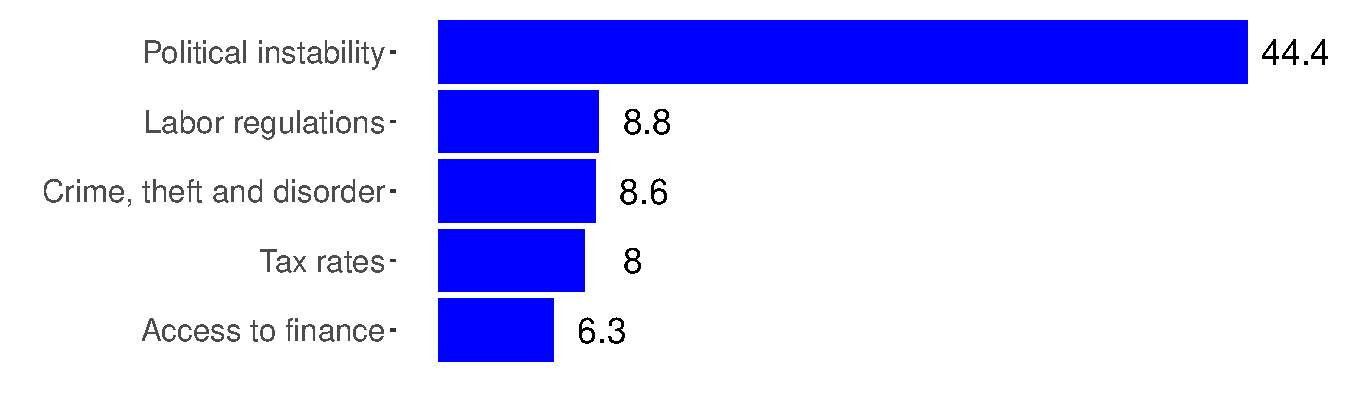
\includegraphics[width=\maxwidth]{figure/top5constraintsES-1} 

}



      %\vspace*{-0.7cm}
      \hspace*{0.3cm} \raggedright\footnotesize{\href{https://www.enterprisesurveys.org/data}{Source: Enterprise Survey 2012}}
    \end{minipage}
    \begin{minipage}[c]{0.49\textwidth} % top 5 constraints WEF
      \center{\color{blue!50!black} \textbf{Top 5 constraints according to WEF 2015 survey \\ \footnotesize(\% respondants among 88 executives)}}


{\centering 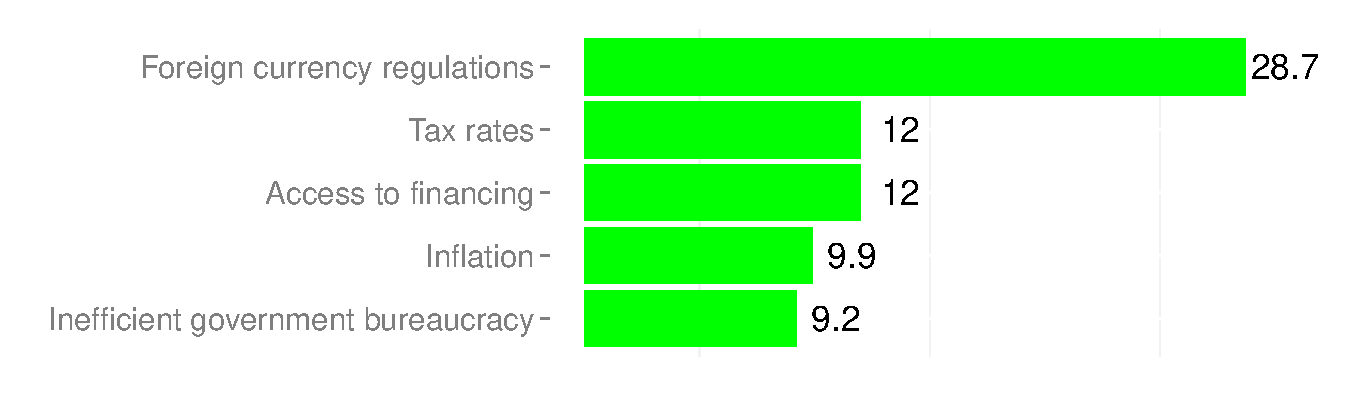
\includegraphics[width=\maxwidth]{figure/top5constraintsWEF-1} 

}



    %\vspace*{-0.7cm}
    \hspace*{0.3cm} \raggedright\footnotesize{\href{http://www.weforum.org/reports/global-competitiveness-report-2015-2016}{Source: WEF Global Competitiveness Report 2015}}
    \end{minipage}
  \end{minipage}
\end{minipage}

% \vspace{+8ex}
% {\color{blue!50!white}\noindent\makebox[\linewidth]{\rule{18cm}{0.3pt}}} % horiz line

% \vspace{+2ex}
% \begin{minipage}[c]{0.33\textwidth}
%   \hspace*{+0.3cm} \includegraphics[width=4cm,left]{/Users/asanchez3/shinyTCMN/www/wb_logo.jpg}
%   %\hspace*{+0.3cm} \includegraphics[width=4cm,left]{/Users/asanchez3/shinyTCMN/www/wb_logo.png}
% \end{minipage}
% \begin{minipage}[c]{0.65\textwidth}
%   \vspace*{-0.4cm}
%   \raggedleft{\color{white!40!black} \footnotesize TRADE AND COMPETITIVENESS MONITORING NOTE - UPDATED} 
%   %month year}
% \end{minipage}

%%%%%%%%%%%%%%%%%%%%%%%%%%%%%%%%%%%
%%%%%% Operations section %%%%%%%%%
%%%%%%%%%%%%%%%%%%%%%%%%%%%%%%%%%%%
\newpage
%%%%%%%%%%%%%%%% PAGE 3 %%%%%%%%%%%%%%%%%%%

%World Bank logo and TCMN branding
\begin{figure}
  \vspace{-3ex} % move up this figure
  \hspace{-7ex} % move left this figure
  \includegraphics[width=5cm]{/Users/asanchez3/shinyTCMN/www/wb_logo_background.png}
\end{figure}
\begin{figure}
  \begin{minipage}[t]{0.99\textwidth} % top section
      \vspace{-30ex}
      \hspace{-2ex}
      \raggedright{\includegraphics[width=5.5cm,right]{/Users/asanchez3/shinyTCMN/www/TC_snapshots_operations.png}}
  \end{minipage}
\end{figure}
%
%%%% Macro Indicators
\begin{minipage}[t]{0.99\textwidth} % top section
  \vspace{-1.5cm}
  \begin{minipage}[c]{0.36\textwidth} 
    \begin{minipage}[c]{0.28\textwidth} % flag
      \includegraphics[width=1.2cm,height=1.2cm]{/Users/asanchez3/shinyTCMN/www/RU.png}
    \end{minipage}
    \begin{minipage}[c]{0.70\textwidth} % Country name
      \section*{\color{blue!40!black}Russian Federation}
    \end{minipage}
  \end{minipage}
  \begin{minipage}[c]{0.63\textwidth}
  %  \begin{flushleft}  
  %    \center{\color{blue!20!black} \textbf{\Large T\&C Product Line Operations Board Approved On or After FY14}}
  %  \end{flushleft} 
  \end{minipage}  
\end{minipage} % end top section

%\begin{minipage}[b]{0.99\textwidth} % main body
  \raggedright{\color{white!30!blue} \textbf{\Large SCD/CPF}}
    \begin{minipage}[c]{0.99\textwidth}  
      \vspace*{0.2cm}
      \raggedright{\color{white!30!blue} \textbf{\large Most Recent}}
      \vspace*{0.3cm}
      
% latex table generated in R 3.2.2 by xtable 1.7-4 package
% Tue May 31 10:59:16 2016
\scalebox{0.85}{
\begin{tabular}{>{\raggedright}p{5in}ll}
 Product & Document Date &  \\ 
  \hline
Russian Federation - Country Partnership Strategy for the period 2012-2016 & 2011-12-22 &  \\ 
  \end{tabular}
}

      \vspace*{0.5cm}
    \end{minipage}
    
    \begin{minipage}[c]{0.99\textwidth} % imports/exports
      \vspace*{0.2cm}
      \raggedright{\color{white!30!blue} \textbf{\large Planned}}
      \vspace*{0.3cm}
      
% latex table generated in R 3.2.2 by xtable 1.7-4 package
% Tue May 31 10:59:16 2016
\scalebox{0.85}{
\begin{tabular}{>{\raggedright}p{5in}lll}
 Product & Concept Review Date & Board Date &  \\ 
  \hline
None &  &  &  \\ 
  \end{tabular}
}

      \vspace*{0.5cm}
    \end{minipage}
%\end{minipage}
  
\vspace*{0.5cm}
\raggedright{\color{white!30!blue} \textbf{\Large WB Lending Pipeline}}
\begin{minipage}[b]{0.99\textwidth} % overview tables
  \begin{minipage}[c]{0.99\textwidth}  
    \vspace*{0.5cm}
% latex table generated in R 3.2.2 by xtable 1.7-4 package
% Tue May 31 10:59:16 2016
{\scriptsize
\scalebox{0.85}{
\begin{tabular}{l>{\raggedright}p{1in}>{\raggedright}p{1in}>{\raggedright}p{0.5in}>{\raggedright}p{0.5in}>{\raggedright}p{0.5in}>{\raggedright}p{0.6in}>{\raggedright}p{0.5in}>{\raggedright}p{0.5in}>{\raggedleft}p{0.5in}>{\raggedleft}p{0.5in}l}
 Project ID & Project Name & Team Leader & Approval Date & Lending Inst. Type & Begin Appraisal & Commitment (US\$M) & Latest Sort Overall Risk Rating & FY Expenses (US\$K) & Cum Expenses (US\$K) & FY Prob &  \\ 
  \hline
P147011 & Russia SEZ Enhancement Project & Ljudmilla V. Poznanskaya & 2018-09-25 & IPF & 2017-07-11 & 132 & --- & 41 & 231 & C &  \\ 
  \end{tabular}
}
}

    \vspace*{0.5cm}
  \end{minipage}
    
  \raggedright{\color{white!30!blue} \textbf{\Large WB Portfolio}}
  \begin{minipage}[c]{0.99\textwidth} % imports/exports
    \vspace*{0.2cm}
    \raggedright{\color{white!30!blue} \textbf{\large Active}}
    \vspace*{0.3cm}
      
% latex table generated in R 3.2.2 by xtable 1.7-4 package
% Tue May 31 10:59:16 2016
{\footnotesize
\scalebox{0.85}{
\begin{tabular}{l>{\raggedright}p{1in}>{\raggedright}p{1in}>{\raggedright}p{0.5in}>{\raggedright}p{0.5in}>{\raggedright}p{0.5in}>{\raggedleft}p{0.5in}>{\raggedleft}p{0.5in}>{\raggedright}p{0.4in}>{\raggedright}p{0.4in}>{\raggedright}p{0.4in}>{\raggedleft}p{0.4in}l}
 Project ID & Project Name & Team Leader & Approval Date & Lending Inst. Type & Closing Date & Commitment (US\$M) & Undisbursed Balance (US\$M) & Project Rating DO & Project Rating IP & Overall Risk & Months in Problem Status &  \\ 
  \hline
None &  &  &  &  &  &  &  &  &  &  &  &  \\ 
  \end{tabular}
}
}

    \vspace*{0.5cm}
  \end{minipage}
     
  \begin{minipage}[c]{0.99\textwidth} % imports/exports 
    \raggedright{\color{white!30!blue} \textbf{\large Closed}}
    \vspace*{0.5cm}
      
% latex table generated in R 3.2.2 by xtable 1.7-4 package
% Tue May 31 10:59:16 2016
{\footnotesize
\scalebox{0.85}{
\begin{tabular}{l>{\raggedright}p{1.5in}>{\raggedright}p{1in}>{\raggedright}p{0.5in}>{\raggedright}p{0.5in}>{\raggedright}p{0.5in}>{\raggedleft}p{0.6in}>{\raggedright}p{0.5in}>{\raggedright}p{0.5in}>{\raggedright}p{0.5in}l}
 Project ID & Project Name & Team Leader & Approval Date & Lending Inst. Type & Closing Date & Commitment (US\$M) & Project Rating DO & Project Rating IP & IEG Outcome Rating &  \\ 
  \hline
None &  &  &  &  &  &  &  &  &  &  \\ 
  \end{tabular}
}
}

    \vspace*{0.5cm}
  \end{minipage}
     
\end{minipage}
 
 \newpage
%%%%%%%%%%%%%%%% PAGE 2 %%%%%%%%%%%%%%%%%%%
\begin{minipage}[t]{0.99\textwidth}
  \raggedright{\color{white!30!blue} \textbf{\Large WB ASA}}

  \begin{minipage}[b]{0.99\textwidth}
    \vspace*{0.2cm}
    \raggedright{\color{white!30!blue} \textbf{\large Active}}
    \vspace*{0.3cm}
  
% latex table generated in R 3.2.2 by xtable 1.7-4 package
% Tue May 31 10:59:16 2016
{\scriptsize
\scalebox{0.85}{
\begin{tabular}{l>{\raggedright}p{1in}>{\raggedright}p{1in}>{\raggedright}p{0.6in}>{\raggedright}p{0.6in}>{\raggedright}p{0.4in}>{\raggedright}p{0.4in}>{\raggedleft}p{0.6in}>{\raggedleft}p{0.6in}>{\raggedleft}p{0.6in}>{\raggedleft}p{0.6in}l}
 Task ID & Task Name & Team Leader & Concept Approval Date & Output Approval Date & Product Line & RAS (Y/N) & Current Expenditure BB (US\$K) & Current Expenditure Total (US\$K) & Lifetime Expenditure BB (US\$K) & Lifetime Expenditure Total (US\$K) &  \\ 
  \hline
P159701 & RAS Investment Climate Reform Advisory 4 & Sylvie K. Bossoutrot & --- & 2018-01-31 & TA & Y & --- &  0 &  --- &   0 &  \\ 
  P145769 & Russia Innovation Support Program & Ljudmilla V. Poznanskaya & 2013-06-18 & 2017-06-30 & PA & N & 40 & 40 & 226 & 218 &  \\ 
  P146625 & Programmatic Support to Microeconomic Re & Ljudmilla V. Poznanskaya & 2013-10-13 & 2017-06-30 & PA & N & 14 & 14 & 277 & 277 &  \\ 
  P147345 & Investment Climate TA & Sylvie K. Bossoutrot & 2013-11-19 & 2017-06-30 & PA & N & 30 & 30 &  30 &  30 &  \\ 
  P149156 & Investment Climate reform support & Sylvie K. Bossoutrot & --- & 2017-06-30 & TA & N & 59 & 59 & 486 & 486 &  \\ 
  P160041 & Russia Cluster Program Assessment & Ljudmilla V. Poznanskaya & --- & 2017-06-30 & TA & N & 30 & 30 &  30 &  30 &  \\ 
  \end{tabular}
}
}

     \vspace*{0.2cm}
  \end{minipage}

  \begin{minipage}[b]{0.99\textwidth}
    \vspace*{0.2cm}
    \raggedright{\color{white!30!blue} \textbf{\large Closed}}
    \vspace*{0.3cm}
       
% latex table generated in R 3.2.2 by xtable 1.7-4 package
% Tue May 31 10:59:16 2016
{\scriptsize
\scalebox{0.85}{
\begin{tabular}{l>{\raggedright}p{1in}>{\raggedright}p{1in}>{\raggedright}p{0.6in}>{\raggedright}p{0.6in}>{\raggedright}p{0.4in}>{\raggedright}p{0.4in}>{\raggedleft}p{0.6in}>{\raggedleft}p{0.6in}>{\raggedleft}p{0.6in}>{\raggedleft}p{0.6in}l}
 Task ID & Task Name & Team Leader & Concept Approval Date & Output Approval Date & Product Line & RAS (Y/N) & Current Expenditure BB (US\$K) & Current Expenditure Total (US\$K) & Lifetime Expenditure BB (US\$K) & Lifetime Expenditure Total (US\$K) &  \\ 
  \hline
P149077 & RU RAS InnObs Stage 2\_Krasnoyarsk region & Ljudmilla V. Poznanskaya & --- & 2016-06-30 & TA & Y &  27 &  27 &    76 &    76 &  \\ 
  P153383 & Investment Climate Reform Advisory (III) & Sylvie K. Bossoutrot & --- & 2016-05-20 & TA & Y & 139 & 139 &   160 &   160 &  \\ 
  P148010 & RU RAS InnObs Stage 2\_Novosibirsk region & Ljudmilla V. Poznanskaya & --- & 2015-12-30 & TA & Y &   0 &   0 &   120 &   120 &  \\ 
  P149075 & RU RAS InnObs Stage 2\_Tomsk Region & Ljudmilla V. Poznanskaya & --- & 2015-10-11 & TA & Y &   0 &   0 &    19 &    19 &  \\ 
  P148944 & Investment promotion for Sverdlovsk reg. & Sylvie K. Bossoutrot & --- & 2015-06-24 & TA & Y &   0 &   0 &    46 &    46 &  \\ 
  P150491 & Competition policy capacity building & Alvaro S. Gonzalez & --- & 2015-06-24 & TA & N &  --- &   0 &    --- &     0 &  \\ 
  P147373 & Russia Post WTO Accession TA & Birgit Hansl & 2014-01-17 & 2015-06-23 & TA & N &  --- &   0 &   127 &   127 &  \\ 
  P149337 & Khanty-Mansiysk Gas Cluster Development & Thomas Edward Haven & 2014-01-24 & 2015-06-23 & TA & Y &   0 &   0 &   113 &   113 &  \\ 
  P147989 & Invest. \& Jobs Through Clusters (CIIP) & Jean-Louis Charles Racine & --- & 2014-07-09 & TA & N &  --- &   0 &    --- &   426 &  \\ 
  P133041 & FBS Investment Climate Reform Adviso II & Sylvie K. Bossoutrot & 2012-11-02 & 2014-06-24 & TA & Y &  --- &   0 &   512 &   512 &  \\ 
  P131669 & FBS-18-FY12-RU-Design of a Venture Accel & Jean-Louis Charles Racine & 2012-06-12 & 2014-04-12 & TA & Y &  --- &   0 &    61 &    61 &  \\ 
  P133192 & FBS: TPU Venture Acceleration Network & Jean-Louis Charles Racine & 2012-10-19 & 2014-04-12 & TA & Y &  --- &   0 &    71 &    71 &  \\ 
  P144720 & TA for Economic Diversification & Alvaro Gonzalez & 2013-04-04 & 2013-06-26 & TA & N &  --- &   0 &   130 &   130 &  \\ 
  P127548 & FBS-17-FY12 Russia Innovation Support & Jean-Louis Charles Racine & 2011-09-16 & 2013-06-25 & TA & Y &   0 &   0 & 1,404 & 1,404 &  \\ 
  P130255 & FBS Tatarstan IP Commercialization & Jean-Louis Charles Racine & 2012-01-17 & 2013-06-18 & TA & Y &  --- &   0 &   167 &   167 &  \\ 
  P129379 & FBS-07-FY12 Tomsk Innovation Strategy & Jean-Louis Charles Racine & 2012-01-17 & 2013-06-08 & TA & Y &  --- &   0 &    75 &    75 &  \\ 
  P129336 & FBS - Novosibirsk Innovation & Jean-Louis Charles Racine & 2011-11-16 & 2012-06-27 & TA & Y &  --- &   0 &    82 &    82 &  \\ 
  P127732 & WTO Monitoring & Birgit Hansl & --- & 2012-06-20 & TA & N &  --- &   0 &    29 &    29 &  \\ 
  P109731 & Regional Competitiveness in Russia & Gjorgjija Petkoski & 2007-10-19 & 2009-06-30 & TE & N &  --- &   0 &    35 &    35 &  \\ 
  P110976 & Russia:  Trade Policy and WTO Accession & Gianni Zanini & 2008-02-20 & 2009-06-30 & TE & N &  --- &   0 &    82 &    82 &  \\ 
  P095097 & G-8 ADV SERVS/TA & Andrei R. Markov & --- & 2007-01-16 & TA & N &  --- &   0 &   455 &   455 &  \\ 
  P102382 & Building Institutions for Evidence Based & Gianni Zanini & --- & 2006-10-27 & TE & N &  --- &   0 &    25 &    25 &  \\ 
  P096166 & Russia Trade Policy \& WTO Accession TOT & Gianni Zanini & --- & 2006-03-24 & TE & N &  --- &   0 &    88 &   117 &  \\ 
  P099387 & Youth Forum:  Russia's Accession to WTO & Gianni Zanini & --- & 2005-12-12 & TE & N &  --- &   0 &    --- &     0 &  \\ 
  P070403 & WTO (TA) & John Litwack & --- & 2005-06-15 & TA & N &  --- &   0 &   637 &   637 &  \\ 
  P082058 & (LKD)PPIAF:  RU Universal AccessTelecom & Gareth Locksley & --- & 2005-06-01 & PT & N &  --- &   0 &   128 &   386 &  \\ 
  P094821 & SPECIAL ECON ZONES TA & Sylvie K. Bossoutrot & --- & 2005-06-01 & TA & N &  --- &   0 &    13 &    13 &  \\ 
  P089264 & Russia WTO Accession course & Carsten Fink & --- & 2005-04-08 & TE & N &  --- &   0 &    87 &   110 &  \\ 
  \end{tabular}
}
}

    \vspace*{0.5cm}
  \end{minipage}

  \raggedright{\color{white!30!blue} \textbf{\Large IFC ASA}}
  \begin{minipage}[b]{0.99\textwidth}
    \vspace*{0.2cm}
    \raggedright{\color{white!30!blue} \textbf{\large Active}}
    \vspace*{0.3cm}
  
% latex table generated in R 3.2.2 by xtable 1.7-4 package
% Tue May 31 10:59:16 2016
{\footnotesize
\scalebox{0.85}{
\begin{tabular}{l>{\raggedright}p{1.6in}>{\raggedright}p{1.5in}>{\raggedright}p{0.7in}>{\raggedright}p{0.7in}>{\raggedleft}p{0.7in}>{\raggedleft}p{0.7in}>{\raggedleft}p{0.7in}l}
 Project ID & Project Name & Team Leader & IP Approval Date & Expected End Date & Approval Value (in US\$K) & Total Expenditures (in US\$K) & Current FY Expenditure (in US\$K) &  \\ 
  \hline
None &  &  &  &  &  &  &  &  \\ 
  \end{tabular}
}
}

    \vspace*{0.2cm}
  \end{minipage}

  \raggedright{\color{white!30!blue} \textbf{\large Pipeline}}
  \vspace*{0.3cm}
  
% latex table generated in R 3.2.2 by xtable 1.7-4 package
% Tue May 31 10:59:16 2016
{\footnotesize
\scalebox{0.85}{
\begin{tabular}{l>{\raggedright}p{1.6in}>{\raggedright}p{1.5in}>{\raggedright}p{0.7in}>{\raggedright}p{0.7in}>{\raggedleft}p{0.7in}>{\raggedleft}p{0.7in}>{\raggedleft}p{0.7in}l}
 Project ID & Project Name & Team Leader & IP Approval Date & Expected End Date & Approval Value (in US\$K) & Total Expenditures (in US\$K) & Current FY Expenditure (in US\$K) &  \\ 
  \hline
None &  &  &  &  &  &  &  &  \\ 
  \end{tabular}
}
}

  \vspace*{0.2cm}
\end{minipage}

\begin{minipage}[b]{0.99\textwidth}
  \raggedright{\color{white!30!blue} \textbf{\large Closed}}
  \vspace*{0.3cm}
  
% latex table generated in R 3.2.2 by xtable 1.7-4 package
% Tue May 31 10:59:16 2016
{\scriptsize
\scalebox{0.85}{
\begin{tabular}{l>{\raggedright}p{1.6in}>{\raggedright}p{1.5in}>{\raggedright}p{0.7in}>{\raggedright}p{0.7in}>{\raggedleft}p{0.7in}>{\raggedleft}p{0.7in}>{\raggedleft}p{0.7in}l}
 Project ID & Project Name & Team Leader & IP Approval Date & Expected End Date & Approval Value (in US\$K) & Total Expenditures (in US\$K) & Current FY Expenditure (in US\$K) &  \\ 
  \hline
27441 & Russian Federation -- BEE improvement in Republic of Tatarstan & Artemiev, Igor E. & 2008-09-05 & 2009-12-31 &  17 & 192 & 0 &  \\ 
  555505 & Subnational Doing Business in Russia & Artemiev, Igor E. & 2007-04-12 & 2009-10-30 & 464 & 220 & 0 &  \\ 
  551525 & Russia--removing admin. barriers for investment, business development in republics of N. Caucasus & Artemiev, Igor E. & 2006-11-30 & 2010-03-31 & 689 & 474 & 0 &  \\ 
  538794 & Removal of Administrative Barriers in Magadan City & Pepper, Roy & 2005-09-01 & 2006-09-30 & 133 & 135 & 0 &  \\ 
  538787 & Removal of Administrative  Barriers-Perm Oblast & Coolidge, Jacqueline & 2005-08-31 & --- &   0 &   0 & 0 &  \\ 
  538784 & Removal of Admin Barriers-Kaliningrad Oblast & Coolidge, Jacqueline & 2005-08-30 & --- &   0 &   0 & 0 &  \\ 
  538431 & Review of the Special Economic Zone Law & Akinci, Gokhan & 2005-08-22 & --- &   0 &   0 & 0 &  \\ 
  538705 & Removal of Admin Barriers-Nizhny Novgorod & Pepper, Roy & 2005-08-22 & --- &   0 &   0 & 0 &  \\ 
  538800 & Removal of Admin Barriers-Leningrad Oblast & Pepper, Roy & 2005-08-22 & 2006-09-30 & 179 & 201 & 0 &  \\ 
  538751 & Monitoring the Impact of Reform on Locating Procedures & Kisunko, Gregory & 2005-08-18 & --- &   0 &   0 & 0 &  \\ 
  538767 & Legislative Reform of Locating Procedures & Coolidge, Jacqueline & 2005-08-17 & --- &   0 &   0 & 0 &  \\ 
  538817 & Pilot Survey of "Runaway Investors" (small project) & Coolidge, Jacqueline & 2005-08-17 & --- &   0 &   0 & 0 &  \\ 
  521687 & Irkutsk Admin. Barrier - Russia & Artemiev, Igor E. & 2005-08-16 & 2007-09-24 & 183 & 207 & 0 &  \\ 
  521688 & Rostov Admin. Barriers - Russia & Artemiev, Igor E. & 2005-08-15 & 2007-09-24 & 183 & 190 & 0 &  \\ 
  538788 & Sakhalin Oblast: Study of Administrative Barriers to Investment & Artemiev, Igor E. & 2005-08-15 & 2005-12-31 & 110 & 109 & 0 &  \\ 
  522071 & Russian Federation, Tomsk Oblast: Monitoring of Administrative Barriers Reforms & Ponomareva, Tatyana & 2005-08-11 & 2007-07-17 &  90 &  85 & 0 &  \\ 
  530760 & Market Assesment and Technical Study for Russian Steel Sector & Alimardanov, Rufat & 2005-07-01 & --- &   0 &   0 & 0 &  \\ 
  523179 & Action Plan to Establish an Independent Telecom Regulatory Body & Chow, Stephen & 2005-06-24 & --- &   0 &   0 & 0 &  \\ 
  535286 & Survey of the Fish Industry in Russia & Luyt, Ian & 2005-06-16 & --- &   0 &   0 & 0 &  \\ 
  \end{tabular}
}
}

  \vspace*{0.2cm}
\end{minipage}
%%%%%%%%%%%%%%%% END OF DOCUMENT %%%%%%%%%%%%%%%%%%%
\end{document}
